%%%%%%%%%%%%%%%%%%%%%%%%%%%%%%%%%%%%%%%%%%%%%%%%%%%%%%%%%%%%%%%%%%%%%%%%%
%  Zawartość: Główny plik szablonu pracy dyplomowej (magisterskiej/inżynierskiej).
%  Opracował: Tomasz Kubik <tomasz.kubik@pwr.edu.pl>
%  Data: kwiecień 2016
%  Wersja: 0.2
%%%%%%%%%%%%%%%%%%%%%%%%%%%%%%%%%%%%%%%%%%%%%%%%%%%%%%%%%%%%%%%%%%%%%%%%%

\documentclass[a4paper,onecolumn,oneside,12pt,extrafontsizes]{memoir}
% W celu przygotowania wydruku do archiwum należy przesłonić komendę powyższą
% dwoma poniższymi komendami:
%\documentclass[a4paper,onecolumn,twoside,10pt]{memoir} 
%\renewcommand{\normalsize}{\fontsize{8pt}{10pt}\selectfont}

%\usepackage[cp1250]{inputenc} % jeśli kodowanie edytowanych plików to cp1250 
\usepackage[utf8]{inputenc} % jeśli kodowanie edytowanych plików to UTF8
\usepackage[T1]{fontenc}
\usepackage[polish]{babel}
%\DisemulatePackage{setspace}
\usepackage{setspace}
\usepackage{tabularx}
\usepackage{color,calc}
\usepackage{float}
%\usepackage{soul} % pakiet z komendami do podkreślania tekstu

\usepackage{ebgaramond} % pakiet z czcionkami garamond, potrzebny tylko do strony tytułowej, musi wystąpić przed pakietem tgtermes

%% Aby uzyskać polskie literki w pdfie (a nie zlepki) korzystamy z pakietu czcionek tgterms. 
%% W pakiecie tym są zdefiniowane klony czcionek Times o kształtach: normalny, pogrubiony, italic, italic pogrubiony.
%% W pakiecie tym brakuje czcionki o kształcie: slanted (podobny do italic). 
%% Jeśli w dokumencie gdzieś zostanie zastosowana czcionka slanted (np. po użyciu komendy \textsl{}), to
%% latex dokona podstawienia na czcionkę standardową i zgłosi to w ostrzeżeniu (warningu).
%% Ponadto tgtermes to czcionka do tekstu. Wszelkie matematyczne wzory będą sformatowane domyślną czcionką do wzorów.
%% Jeśli wzory mają być sformatowane z wykorzystaniem innych czcionek, trzeba to jawnie zadeklarować.

%% Po zainstalowaniu pakietu tgtermes może będzie trzeba zauktualizować informacje 
%% o dostępnych fontach oraz mapy. Można to zrobić z konsoli (jako administrator)
%% initexmf --admin --update-fndb
%% initexmf --admin --mkmaps

\usepackage{tgtermes}   
\renewcommand*\ttdefault{txtt}

% We wcześniejszej wersji szablonu korzystano z innych czcionek. Dla celów historycznych pozostawiono je w komentarzu
%\usepackage{mathptmx} % pakiet będący następcą pakietów times and mathptm, niestety polskie literki są zlepkami
%\usepackage{newtxtext,newtxmath} % pakiety dostarczające Times dla tekstów i wzorów matematycznych,  
%                                  rozwiązuje problemy występujące w mathptmx, ale wymaga zainstalowania
%                                  dodatkowych pakietów oraz uruchomienia updmap (konsola administratora)
%                                  niestety polskie literki są zlepkami
%\usepackage{newtxmath,tgtermes} % można też połączyć czcionki do tekstu i czcionki do wzorów

\usepackage{listings} % pakiet do prezentacji kodu. 
%Wcześniej był problem z polskimi znakami w otoczeniu lstlisting, stąd pozostawiono w komentarzu zastosowane wtedy rozwiązanie: 
\lstset{literate=%-
{ą}{{\k{a}}}1 {ć}{{\'c}}1 {ę}{{\k{e}}}1 {ł}{{\l{}}}1 {ń}{{\'n}}1 {ó}{{\'o}}1 {ś}{{\'s}}1 {ż}{{\.z}}1 {ź}{{\'z}}1 {Ą}{{\k{A}}}1 {Ć}{{\'C}}1 {Ę}{{\k{E}}}1 {Ł}{{\L{}}}1 {Ń}{{\'N}}1 {Ó}{{\'O}}1 {Ś}{{\'S}}1 {Ż}{{\.Z}}1 {Ź}{{\'Z}}1 }%{\ \ }{{\ }}1}

% Choć możliwe jest zastosowanie różnych pakietów formatujących tabele, zaleca się tego nie robić.
%\usepackage{longtable}
%\usepackage{ltxtable}
%\usepackage{tabulary}

%%%%%%%%%%%%%%%%%%%%%%%%%%%%%%%%%%%%%%%%%%%%%%%%%%%
%% Ustawienia odpowiedzialne za sposób łamania dokumentu
%% i ułożenie elementów pływających
%%%%%%%%%%%%%%%%%%%%%%%%%%%%%%%%%%%%%%%%%%%%%%%%%%%
%\hyphenpenalty=10000		% nie dziel wyrazów zbyt często
\clubpenalty=10000      %kara za sierotki
\widowpenalty=10000  % nie pozostawiaj wdów
\brokenpenalty=10000		% nie dziel wyrazów między stronami
\exhyphenpenalty=999999		% nie dziel słów z myślnikiem
\righthyphenmin=3			% dziel minimum 3 litery

%\tolerance=4500
%\pretolerance=250
%\hfuzz=1.5pt
%\hbadness=1450

\renewcommand{\topfraction}{0.95}
\renewcommand{\bottomfraction}{0.95}
\renewcommand{\textfraction}{0.05}
\renewcommand{\floatpagefraction}{0.35}

%%%%%%%%%%%%%%%%%%%%%%%%%%%%%%%%%%%%%%%%%%%%%%%%%%%
%%  Ustawienia rozmiarów: tekstu, nagłówka i stopki, marginesów
%%  dla dokumentów klasy memoir 
%%%%%%%%%%%%%%%%%%%%%%%%%%%%%%%%%%%%%%%%%%%%%%%%%%%
\setlength{\headsep}{10pt} 
\setlength{\headheight}{13.6pt} % wartość baselineskip dla czcionki 11pt tj. \small wynosi 13.6pt
\setlength{\footskip}{\headsep+\headheight}
\setlength{\uppermargin}{\headheight+\headsep+1cm}
\setlength{\textheight}{\paperheight-\uppermargin-\footskip-1.5cm}
\setlength{\textwidth}{\paperwidth-5cm}
\setlength{\spinemargin}{2.5cm}
\setlength{\foremargin}{2.5cm}
\setlength{\marginparsep}{2mm}
\setlength{\marginparwidth}{2.3mm}
%\settrimmedsize{297mm}{210mm}{*}
%\settrims{0mm}{0mm}	
\checkandfixthelayout[fixed] % konieczne, aby się dobrze wszystko poustawiało
%%%%%%%%%%%%%%%%%%%%%%%%%%%%%%%%%%%%%%%%%%%%%%%%
%%  Ustawienia odległości linii, wcięć, odstępów
%%%%%%%%%%%%%%%%%%%%%%%%%%%%%%%%%%%%%%%%%%%%%%%%
\linespread{1}
%\linespread{1.241}
\setlength{\parindent}{14.5pt}
%\setbeforesecskip{10pt plus 0.5ex}%{-3.5ex \@plus -1ex \@minus -.2ex}
%\setaftersecskip{10pt plus 0.5ex}%\onelineskip}
%\setbeforesubsecskip{8pt plus 0.5ex}%{-3.5ex \@plus -1ex \@minus -.2ex}
%\setaftersubsecskip{8pt plus 0.5ex}%\onelineskip}
%\setlength\floatsep{6pt plus 2pt minus 2pt} 
%\setlength\intextsep{12pt plus 2pt minus 2pt} 
%\setlength\textfloatsep{12pt plus 2pt minus 2pt} 

%%%%%%%%%%%%%%%%%%%%%%%%%%%%%%%%%%%%%%%%%%%%%%%%%%%
%%  Pakiety i komendy zastosowane tylko do zamieszczenia informacji o użytych komendach i fontach
%%  Normalnie nie są potrzebne, można je zamarkować podczas redakcji pracy
%%%%%%%%%%%%%%%%%%%%%%%%%%%%%%%%%%%%%%%%%%%%%%%%%%%
%\usepackage{memlays}     % extra layout diagrams, zastosowane w szblonie do 'debuggowania', używa pakietu layouts
%\usepackage{layouts}
%\usepackage{printlen} % pakiet do wyświetlania wartości zdefiniowanych długości, stosowany do 'debuggowania'
%\uselengthunit{pt}
%\makeatletter
%\newcommand{\showFontSize}{\f@size pt} % makro wypisujące wielkość bieżącej czcionki
%\makeatother
% do pokazania ramek można byłoby użyć:
%\usepackage{showframe} 


%%%%%%%%%%%%%%%%%%%%%%%%%%%%%%%%%%%%%%%%%%%%%%%%%%%
%%  Formatowanie list wyliczeniowych, wypunktowań i własnych otoczeń
%%%%%%%%%%%%%%%%%%%%%%%%%%%%%%%%%%%%%%%%%%%%%%%%%%%

% Domyślnie wypunktowania mają zadeklatorowane znaki, które nie występują w tgtermes
% Aby latex nie podstawiał w ich miejsca znaków z czcionki standardowej można zrobić podstawienie:
%    \DeclareTextCommandDefault{\textbullet}{\ensuremath{\bullet}}
%    \DeclareTextCommandDefault{\textasteriskcentered}{\ensuremath{\ast}}
%    \DeclareTextCommandDefault{\textperiodcentered}{\ensuremath{\cdot}}
% Jednak jeszcze lepszym pomysłem jest zdefiniowanie otoczeń z wykorzystaniem enumitem
\usepackage{enumitem} % pakiet pozwalający zarządzać formatowaniem list wyliczeniowych
\setlist{noitemsep,topsep=4pt,parsep=0pt,partopsep=4pt,leftmargin=*} % zadeklarowane parametry pozwalają uzyskać 'zwartą' postać wypunktowania bądź wyliczenia
\setenumerate{labelindent=0pt,itemindent=0pt,leftmargin=!,label=\arabic*.} % można zmienić \arabic na \alph, jeśli wyliczenia mają być z literkami
\setlistdepth{4} % definiujemy głębokość zagnieżdżenia list wyliczeniowych do 4 poziomów
\setlist[itemize,1]{label=$\bullet$}  % definiujemy, jaki symbol ma być użyty w wyliczeniu na danym poziomie
\setlist[itemize,2]{label=\normalfont\bfseries\textendash}
\setlist[itemize,3]{label=$\ast$}
\setlist[itemize,4]{label=$\cdot$}
\renewlist{itemize}{itemize}{4}

%%%http://tex.stackexchange.com/questions/29322/how-to-make-enumerate-items-align-at-left-margin
%\renewenvironment{enumerate}
%{
%\begin{list}{\arabic{enumi}.}
%{
%\usecounter{enumi}
%%\setlength{\itemindent}{0pt}
%%\setlength{\leftmargin}{1.8em}%{2zw} % 
%%\setlength{\rightmargin}{0zw} %
%%\setlength{\labelsep}{1zw} %
%%\setlength{\labelwidth}{3zw} % 
%\setlength{\topsep}{6pt}%
%\setlength{\partopsep}{0pt}%
%\setlength{\parskip}{0pt}%
%\setlength{\parsep}{0em} % 
%\setlength{\itemsep}{0em} % 
%%\setlength{\listparindent}{1zw} % 
%}
%}{
%\end{list}
%}

\makeatletter
\renewenvironment{quote}{
	\begin{list}{}
	{
	\setlength{\leftmargin}{1em}
	\setlength{\topsep}{0pt}%
	\setlength{\partopsep}{0pt}%
	\setlength{\parskip}{0pt}%
	\setlength{\parsep}{0pt}%
	\setlength{\itemsep}{0pt}
	}
	}{
	\end{list}}
\makeatother

%%%%%%%%%%%%%%%%%%%%%%%%%%%%%%%%%%%%%%%%%
%%  Pakiet do generowania indeksu (ważne, aby wstawić przed hyperref)
%%%%%%%%%%%%%%%%%%%%%%%%%%%%%%%%%%%%%%%%%
%\DisemulatePackage{imakeidx}
%\usepackage[makeindex,noautomatic]{imakeidx} % tutaj mówimy, żeby indeks nie generował się automatycznie, 

%\usepackage[noautomatic]{imakeidx} 
\makeindex

\makeatletter
%%%\renewenvironment{theindex}
							 %%%{\vskip 10pt\@makeschapterhead{\indexname}\vskip -3pt%
								%%%\@mkboth{\MakeUppercase\indexname}%
												%%%{\MakeUppercase\indexname}%
								%%%\vspace{-3.2mm}\parindent\z@%
								%%%\renewcommand\subitem{\par\hangindent 16\p@ \hspace*{0\p@}}%%
								%%%\phantomsection%
								%%%\begin{multicols}{2}
								%%%%\thispagestyle{plain}
								%%%\parindent\z@                
								%%%%\parskip\z@ \@plus .3\p@\relax
								%%%\let\item\@idxitem}
							 %%%{\end{multicols}\clearpage}
%%%
\makeatother


\usepackage{ifpdf}
%\newif\ifpdf \ifx\pdfoutput\undefined
%\pdffalse % we are not running PDFLaTeX
%\else
%\pdfoutput=1 % we are running PDFLaTeX
%\pdftrue \fi
\ifpdf
 \usepackage[pdftex,bookmarks,breaklinks,unicode]{hyperref}
 \usepackage[pdftex]{graphicx}
 \DeclareGraphicsExtensions{.pdf,.jpg,.mps,.png}
\pdfcompresslevel=9
\pdfoutput=1
\makeatletter
\AtBeginDocument{
  \hypersetup{
	pdfinfo={
    Title = {\@title},
    Author = {\@author},
    Subject={},
    Keywords={słowa kluczowe},
  }}
}
\makeatother
\else
\usepackage{graphicx}
\DeclareGraphicsExtensions{.eps,.ps,.jpg,.mps,.png}
\fi
\sloppy


%\graphicspath{{rys01/}{rys02/}}


%%%%%%%%%%%%%%%%%%%%%%%%%%%%%%%%%%%%%%%%%
% Metadane dla pdfa


%\ifpdf
%\pdfinfo{
   %/Author (Nicola Talbot)
   %/Title  (Creating a PDF document using PDFLaTeX)
   %/CreationDate (D:20040502195600)
   %/ModDate (D:\pdfdate)
   %/Subject (PDFLaTeX)
   %/Keywords (PDF;LaTeX)
%}
%\fi

% Deklaracja głębokościu numeracji
\setcounter{secnumdepth}{2}
\setcounter{tocdepth}{2}
\setsecnumdepth{subsection} % activating subsubsec numbering in doc


% Kropki po numerach sekcji
\makeatletter
\def\@seccntformat#1{\csname the#1\endcsname.\quad}
\def\numberline#1{\hb@xt@\@tempdima{#1\if&#1&\else.\fi\hfil}}
\makeatother

\renewcommand{\chapternumberline}[1]{#1.\quad}
\renewcommand{\cftchapterdotsep}{\cftdotsep}

%\definecolor{niceblue}{rgb}{.168,.234,.671}

% Czcionka do podpisów tabel i rysunków
\captionnamefont{\small}
\captiontitlefont{\small}
% makro pozwalające zmienić sposób wypisywania rozdziału
%\def\printchaptertitle##1{\fonttitle \space \thechapter.\space ##1} 

%\usepackage{ltcaption}
% The ltcaption package supports \CaptionLabelFont & \CaptionTextFont introduced by the NTG document classes
%\renewcommand\CaptionLabelFont{\small}
%\renewcommand\CaptionTextFont{\small}

% Przedefiniowanie etykiet w podpisach tabel i rysunków
%\AtBeginDocument{% 
        \addto\captionspolish{% 
        \renewcommand{\tablename}{Tab.}% 
}%} 

%\AtBeginDocument{% 
%        \addto\captionspolish{% 
%        \renewcommand{\chaptername}{Rozdział}% 
%}} 

%\AtBeginDocument{% 
        \addto\captionspolish{% 
        \renewcommand{\figurename}{Rys.}% 
}%}


%\AtBeginDocument{% 
        \addto\captionspolish{% 
        \renewcommand{\bibname}{Literatura}% 
}%}

%\AtBeginDocument{% 
        \addto\captionspolish{% 
        \renewcommand{\listfigurename}{Spis rysunków}% 
}%}

%\AtBeginDocument{% 
        \addto\captionspolish{% 
        \renewcommand{\listtablename}{Spis tabel}% 
}%}

%\AtBeginDocument{% 
        \addto\captionspolish

%%%%%%%%%%%%%%%%%%%%%%%%%%%%%%%%%%%%%%%%%%%%%%%%%%%%%%%%%%%%%%%%%%                  
%% Definicje stopek i nagłówków
%%%%%%%%%%%%%%%%%%%%%%%%%%%%%%%%%%%%%%%%%%%%%%%%%%%%%%%%%%%%%%%%%%                  
\addtopsmarks{headings}{%
\nouppercaseheads % added at the beginning
}{%
\createmark{chapter}{both}{shownumber}{}{. \space}
%\createmark{chapter}{left}{shownumber}{}{. \space}
\createmark{section}{right}{shownumber}{}{. \space}
}%use the new settings

\makeatletter
\copypagestyle{outer}{headings}
\makeoddhead{outer}{}{}{\small\itshape\rightmark}
\makeevenhead{outer}{\small\itshape\leftmark}{}{}
\makeoddfoot{outer}{\small\@author:~\@titleShort}{}{\small\thepage}
\makeevenfoot{outer}{\small\thepage}{}{\small\@author:~\@title}
\makeheadrule{outer}{\linewidth}{\normalrulethickness}
\makefootrule{outer}{\linewidth}{\normalrulethickness}{2pt}
\makeatother

% fix plain
\copypagestyle{plain}{headings} % overwrite plain with outer
\makeoddhead{plain}{}{}{} % remove right header
\makeevenhead{plain}{}{}{} % remove left header
\makeevenfoot{plain}{}{}{}
\makeoddfoot{plain}{}{}{}

\copypagestyle{empty}{headings} % overwrite plain with outer
\makeoddhead{empty}{}{}{} % remove right header
\makeevenhead{empty}{}{}{} % remove left header
\makeevenfoot{empty}{}{}{}
\makeoddfoot{empty}{}{}{}


%%%%%%%%%%%%%%%%%%%%%%%%%%%%%%%%%%%%%%%
%% Definicja strony tytułowej 
%%%%%%%%%%%%%%%%%%%%%%%%%%%%%%%%%%%%%%%
\makeatletter
%Uczelnia
\newcommand\uczelnia[1]{\renewcommand\@uczelnia{#1}}
\newcommand\@uczelnia{}
%Wydział
\newcommand\wydzial[1]{\renewcommand\@wydzial{#1}}
\newcommand\@wydzial{}
%Kierunek
\newcommand\kierunek[1]{\renewcommand\@kierunek{#1}}
\newcommand\@kierunek{}
%Specjalność
\newcommand\specjalnosc[1]{\renewcommand\@specjalnosc{#1}}
\newcommand\@specjalnosc{}
%Tytuł po angielsku
\newcommand\titleEN[1]{\renewcommand\@titleEN{#1}}
\newcommand\@titleEN{}
%Tytuł krótki
\newcommand\titleShort[1]{\renewcommand\@titleShort{#1}}
\newcommand\@titleShort{}
%Promotor
\newcommand\promotor[1]{\renewcommand\@promotor{#1}}
\newcommand\@promotor{}

%\usepackage[absolute]{textpos} % zamarkowano, bo ostatecznie wykorzystano otoczenie picture

\def\maketitle{%
  \pagestyle{empty}%
%%\garamond 
	\fontfamily{\ebgaramond@family}\selectfont % na stronie tytułowej czcionka garamond
%%%%%%%%%%%%%%%%%%%%%%%%%%%%%%%%%%%%%	
%% Poniżej, w otoczniu picture, wstawiono tytuł i autora. 
%% Tytuł (z autorem) musi znaleźć się w obszarze 
%% odpowiadającym okienku 110mmx75mm, którego lewy górny róg 
%% jest w położeniu 77mm od lewej i 111mm od górnej  krawędzi strony 
%% (tak wynika z wycięcia na okładce). 
%% Poniższy kod musi być użyty dokładnie w miejscu gdzie jest.
%% Jeśli tytuł nie mieści się w okienku, to należy tak pozmieniać 
%% parametry użytych komend, aby ten przydługi tytuł jednak 
%% upakować go do okienka.
%%
%% Sama okładka (kolorowa strona z wycięciem, do pobrania z dydaktyki) 
%% powinna być przycięta o 3mm od każdej z krawędzi.
%% Te 3mm pewnie zostawiono na ewentualne spady czy też specjalną oprawę.
%%%%%%%%%%%%%%%%%%%%%%%%%%%%%%%%%%%%%	
\newlength{\tmpfboxrule}
\setlength{\tmpfboxrule}{\fboxrule}
\setlength{\fboxsep}{2mm}
\setlength{\fboxrule}{0mm} 
\setlength{\fboxrule}{0.1mm} %% jeśli chcemy zobaczyć ramkę
\setlength{\unitlength}{1mm}
\begin{picture}(0,0)
\put(5,-124){\fbox{
\parbox[c][71mm][c]{104mm}{\centering%\lineskip=34pt 
\fontsize{16pt}{18pt}\selectfont \@title\\[5mm]
\fontsize{16pt}{18pt}\selectfont \@titleEN\\[20mm]
\fontsize{16pt}{18pt}\selectfont AUTOR:\\[2mm]
\fontsize{14pt}{16pt}\selectfont \@author}
}
}
\end{picture}
\setlength{\fboxrule}{\tmpfboxrule} 
%%%%%%%%%%%%%%%%%%%%%%%%%%%%%%%%%%%%%
%% Reszta strony z nazwą uczelni, wydziału, kierunkiem, specjalnością
%% promotorem, oceną pracy, miastem i rokiem
	{\centering%\vspace{-1cm}
		{\fontsize{22pt}{24pt}\selectfont \@uczelnia}\\[0.4cm]
		{\fontsize{22pt}{24pt}\selectfont \@wydzial}\\[0.5cm]
		  \hrule %\vspace*{0.7cm}
	}
{\flushleft\fontsize{14pt}{16pt}\selectfont%
\begin{tabular}{ll}
KIERUNEK: & \@kierunek\\
%SPECJALNOŚĆ: & \@specjalnosc\\
\end{tabular}\\[1.3cm]
}
{\centering
{\fontsize{32pt}{36pt}\selectfont Systemy infromacyjne}\\[0.5cm]
{\fontsize{32pt}{36pt}\selectfont Seminarium}\\[2.5cm]
}
\vfill
\begin{tabularx}{\linewidth}{p{6cm}l}
		&{\fontsize{16pt}{18pt}\selectfont PROWADZĄCY:}\\[2mm] %UWAGA: tutaj jest miejsce na nazwisko promotora pracy
		&{\fontsize{14pt}{16pt}\selectfont \@promotor}\\[10mm]
		&{\fontsize{16pt}{18pt}\selectfont OCENA PRACY:}\\[20mm]
	\end{tabularx}
\vspace{2cm}
\hrule\vspace*{0.3cm}
{\centering
{\fontsize{16pt}{18pt}\selectfont \@date}\\[0cm]
}
%\ungaramond
\normalfont
 \cleardoublepage
}
\makeatother
%%%%%%%%%%%%%%%%%%%%%%%%%%%%%%%%%%%%%%%%%
\usepackage{color}
\lstset{
    numbers=left,
    breaklines=true,
    backgroundcolor=\color[rgb]{0.95,0.95,0.95},
    tabsize=2,
    basicstyle=\ttfamily,
    float,
    literate={\ \ }{{\ }}1
}
\usepackage{lscape}
\bibliographystyle{unsrt}


%%%%%%%%%%%%%%%%%%%%%%%%%%%%%%%%%%%%%%%%%
%%  Metadane dokumentu 
%%%%%%%%%%%%%%%%%%%%%%%%%%%%%%%%%%%%%%%%%
\title{Kierunki rozwoju wyszukiwania obrazów i wideo w sieci Internet}
\titleShort{Kierunki rozwoju wyszukiwania obrazów i wideo w sieci Internet}
%\titleEN{Hand gesture recognition}
\author{Bartosz Kardas}
\uczelnia{POLITECHNIKA WROCŁAWSKA}
\wydzial{WYDZIAŁ INFORMATYKI I ZARZĄDZANIA}
\kierunek{INFORMATYKA}
%\specjalnosc{INŻYNIERIA INTERNETOWA}
\promotor{dr inż. Elżbieta Kukla}
\date{WROCŁAW, 2016}

% Ustawienie odstępu od góry w nienumerowanych rozdziałach oraz wykazach:
% Spis treści, Spis tabel, Spis rysunków, Indeks rzeczowy

%\newlength{\linespace}
%\setlength{\linespace}{-\beforechapskip-\topskip+\headheight+\topsep}
%\makechapterstyle{noNumbered}{%
%\renewcommand\chapterheadstart{\vspace*{\linespace}}
%}

%% powyższa komenda załatwia to, co robią komendy poniższe dla spisów
%\renewcommand*{\tocheadstart}{\vspace*{\linespace}}
%\renewcommand*{\lotheadstart}{\vspace*{\linespace}}
%\renewcommand*{\lofheadstart}{\vspace*{\linespace}}

%%%%%%%%%%%%%%%%%%%%%%%%%%%%%%%%%%%%%%%%%
%                  Początek dokumentu 
%%%%%%%%%%%%%%%%%%%%%%%%%%%%%%%%%%%%%%%%%
%\includeonly{skroty,rozdzial01} % jeśli chcemy kompilować tylko fragmenty, to można tu je wpisać

\begin{document}
% Tutaj można przełączyć odstęp między liniami
%\SingleSpacing
%\OnehalfSpacing
%\DoubleSpacing

%\settypeoutlayoutunit{cm} % do debugowania
%\typeoutstandardlayout    % wypisuje na stdout informacje o ustawieniach
%\maketitle

%\newpage
%\thispagestyle{empty}
%\mbox{}\vfill
%\noindent\begin{tabular}{@{}ll} Opracował: & Tomasz Kubik <tomasz.kubik@pwr.edu.pl>\\
% Data: & maj 2016 
% \end{tabular}\\[15mm]
%\noindent\includegraphics[width=3cm]{by-nc-sa}\newline
%{\normalfont 
%Szablon jest udostępniany na licencji Creative Commons: \emph{Uznanie autorstwa -- Użycie niekomercyjne -- Na tych samych warunkach, 3.0 Polska}, Wrocław 2016. \\[2pt]
%Oznacza to, że wszystkie zawarte  nim treści można kopiować i  wykorzystywać do celów niekomercyjnych, a także tworzyć na ich podstawie utwory zależne pod warunkiem podania autora i~nazwy licencjodawcy oraz udzielania na utwory zależne takiej samej licencji. Tekst licencji jest dostępny pod adresem: \url{http://creativecommons.org/licenses/by-nc-sa/3.0/pl/}.}
\newpage


\chapterstyle{noNumbered}
\pagestyle{outer}
\mbox{}\pdfbookmark[0]{Spis treści}{spisTresci.1}
\tableofcontents* 

\newpage
\mbox{}\pdfbookmark[0]{Spis rysunków}{spisRysunkow.1}
%\addcontentsline{toc}{chapter}{Spis rysunków}
\listoffigures*
\mbox{}\pdfbookmark[0]{Spis tabel}{spisTabel.1}
\listoftables*
\begin{flushleft}

\end{flushleft}

%\chapter*{Skróty}\mbox{}\pdfbookmark[0]{Skróty}{skroty.1}
\label{sec:skroty}
\noindent
\begin{description}
  \item [OGC] (ang.\ \emph{Open Geospatial Consortium}) %-- jednostka arytmetyczno--logiczna
  \item [XML] (ang.\ \emph{eXtensible Markup Language})
  \item [SOAP] (ang.\ \emph{Simple Object Access Protocol})
  \item [WSDL] (ang.\ \emph{Web Services Description Language})
  \item [UDDI] (ang.\ \emph{Universal Description Discovery and Integration})
  \item [GIS] (ang.\ \emph{Geographical Information System})
  \item [SDI] (ang.\ \emph{Spatial Data Infrastructure})
  \item [ISO] (ang.\ \emph{International Standards Organization})
  \item [WMS] (ang.\ \emph{Web Map Service})
  \item [WFS] (ang.\ \emph{Web Feature Service})
  \item [WPS] (ang.\ \emph{Web Processing Service})
  \item [GML] (ang.\ \emph{Geography Markup Language})
  \item [SRG] (ang.\ \emph{Seeded Region Growing})
  \item [SOA] (ang.\ \emph{Service Oriented Architecture })
  \item [IT] (ang.\ \emph{Information Technology })
\end{description}
 %skróty można sobie pominąć
\chapterstyle{default}
\chapter{Naiwny klasyfikator bayesowski - opis}
	\section{Algorytm} \label{algo}
Naiwny klasyfikator bayesowski opiera się na twierdzeniu bayesa o prawdopodobieństwie warunkowym. Słowo 'naiwny' pochodzi od zaadaptowania warunku iż każdy z atrybutów jest od siebie niezależny. W rzeczywistości warunek ten jest ciężki do spełnienia, ale pomimo tego klasyfikator ten charakteryzuję się zaskakująco dobrą skutecznością.

Budowa modelu polega na wyznaczeniu cząstkowych prawdopodobieństw $P(X_i|C)$ wystąpienia danego atrybutu $X_i$ pod warunkiem wystąpienia klasy $C$ oraz na obliczeniu prawdopodobieństw $P(C)$ wystąpienia danej klasy w zbiorze. Następnie w wyniku zastosowania twierdzenia bayesa i opisanej wyżej 'naiwności' można zastosować poniższy wzór służący do klasyfikacji obiektu o atrybutach $x_1, x_2,..., x_n$ za pomocą poniższego wzoru.
$$ predict(x_1, x_2,..., x_n) = argmax_cP(C=c)\prod_{i=1}^{n}P(X_i = x_i | C = c)$$
Innymi słowy, klasyfikacja odbywa się na zasadzie znalezienia wartości maksymalnej z iloczyny wcześniej wyliczonych prawdopodobieństw. 

W implementacji algorytmu często stosuje się wersję z sumą logarytmów prawdopodobieństw, zapewniającą dokładniejsze wyniki dla małych prawdopodobieństw i dużej ilości atrybutów (w wyniku mnożenia i niedokładności liczb zmiennoprzecinkowych można otrzymać zerowe prawdopodobieństwo). 
$$ predict(x_1, x_2,..., x_n) = argmax_c ln( P(C=c) )\sum_{i=1}^{n}ln( P(X_i = x_i | C = c) )$$
	\section{Problem zerowego prawdopodobieństwa}
Podczas nauki klasyfikatora może nastąpić problem zerowego prawdopodobieństwa, w przypadku gdy dana klasa atrybutu nie występuje w parze z klasą. Aby uniknąć tego typu sytuacji należy dodać $1$ do każdego elementu macierzy liczności klasa-atrybut. Metoda ta nazywa się wygładzaniem Laplace'a (ang. Laplace smoothing). Poniżej przedstawiono przykład obliczeniowy ilustrujący działanie metody.

\begin{table}[H]
\centering
\caption{Rozkład danych przed zastosowaniem metody}
\begin{tabular}{ ccc }
 & $C = yes$ & $C = no$ \\
$A = sunny$ & 5 & 3 \\
$A = windy$ & 0 & 0 \\
\end{tabular}
\end{table}
Z powyższej tabeli wynika, że
$$P(A = sunny | C = yes) = \frac{5}{5} = 1$$
$$P(A = windy | C = yes) = \frac{0}{5} = 0$$

Po zastosowaniu powyżej opisanej metody otrzymujemy

\begin{table}[H]
\centering
\caption{Rozkład danych przed zastosowaniem metody}
\begin{tabular}{ ccc }
 & $C = yes$ & $C = no$ \\
$A = sunny$ & 6 & 4 \\
$A = windy$ & 1 & 1 \\
\end{tabular}
\end{table}
Z odpowiadającymi nie zerowymi prawdopodobieństwami.
$$P(A = sunny | C = yes) = \frac{6}{7} $$
$$P(A = windy | C = yes) = \frac{1}{7} $$
	\section{Dane ciągłe, rozkład normalny}
Dla danych ciągłych można także zastosować rozkład Gaussa do obliczenia statystyki. Poniżej przedstawiono wzór na prawdopodobieństwo warunkowe wystąpienia wartości $i$-tego atrybutu $x_i$, pod warunkiem wystąpienia klasy $c$.

$$ P(x_i|c) = \frac{1}{\sigma\sqrt{2\pi}}e^{-\frac{(x_i - \mu)^2}{2\sigma^2}}$$, gdzie\newline
$x_i$ - wartość $i$-tego atrybutu\newline
$x_i$ - klasa\newline
$\mu$ - wartość średnia zbioru wartości $i$-tego atrybutu\newline
$\sigma$ - odchylenie standardowe zbioru wartości $i$-tego atrybutu\newline
\chapter{Dane testowe - charakterystyka}

\section{Seeds}
	\subsection{Opis}
Zbiór zawiera dane dotyczące charakterystki ziaren. Zawiera 3 klasy ziaren: Kama, Rosa and Canadian, po 70 rekordów każdy. Każde z ziaren opisane jest przez 7 atrybutów rzeczywistych. Łącznie 210 rekordów. Każde z ziaren jest opisane, nie posiada brakujących wartości. Zbiór może być wykorzystywany do metod klasyfikacji oraz klasteryzacji.
	\subsection{Dystrybucja klas}
Liczności poszczególnych klas zostały przedstawione w tabeli \ref{dist-seeds}
\begin{table}[H]
\centering
\caption{Dystrybucja klas w zbiorze seeds.}
\label{dist-seeds}
\begin{tabular}{ll}
NAZWA    & LICZNOŚĆ \\
Kama     & 70       \\
Rosa     & 70       \\
Canadian & 70      
\end{tabular}
\end{table}
	\subsection{Atrybuty}
	Poniżej \ref{attr-seeds} przedstawiono opis poszczególnych atrybutów.
\begin{table}[H]
\centering
\caption{Opis atrybutów w zbiorze seeds.}
\label{attr-seeds}
\begin{tabular}{lll}
NAZWA    	& RODZAJ & OPIS \\
Wielkość	& REAL	& area $A$\\
Perymetr	& REAL & perimeter $P$\\
Kompaktowość & REAL & compactness C = $4*pi*A/P^2$\\
Długość		& REAL & length of kernel\\
Szerokość	& REAL & width of kernel\\
Współczynnik asymetrii	& REAL & asymmetry coefficient\\
Długość rowka			& REAL & length of kernel groove 
\end{tabular}
\end{table}

\section{Ecoli}
	\subsection{Opis}
Zbiór zawiera dane dotyczące miejsca lokalizacji białek. Zawiera 8 klas lokalizacji przedstawione w tabeli \ref{dist-ecoli}. Każda z lokalizacji opisana jest przez 5 atrybutów rzeczywistych, 2 binarne, 1 kategoryczny, z czego ostatni jest nazwą konkretnej sekwencji (unikalna dla każdego rekordu). Łącznie 336 rekordów. Każdy z nich jest w pełni opisany, nie posiada brakujących wartości. Zbiór może być wykorzystywany do metod klasyfikacji.
	\subsection{Dystrybucja klas}
	Liczności poszczególnych klas zostały przedstawione w tabeli \ref{dist-ecoli}
\begin{table}[H]
\centering
\caption{Dystrybucja klas w zbiorze ecoli.}
\label{dist-ecoli}
\begin{tabular}{lll}
NAZWA & LICZNOŚĆ & OPIS \\
cp	& 143	& cytoplasm\\
im	& 77	& inner membrane without signal sequence\\
pp	& 52	& perisplasm\\
imU	& 35	& inner membrane, uncleavable signal sequence\\
om	& 20	& outer membrane\\
omL	& 5	 & outer membrane lipoprotein\\
imL	& 2	 & inner membrane lipoprotein\\
imS	& 2	 & inner membrane, cleavable signal sequence
\end{tabular}
\end{table}
	\subsection{Atrybuty}
	Poniżej \ref{attr-ecoli} przedstawiono opis poszczególnych atrybutów.
\begin{table}[H]
\centering
\caption{Opis atrybutów w zbiorze seeds.}
\label{attr-ecoli}
\begin{tabular}{lll}
NAZWA    	& RODZAJ \\
name	& UNIQUE	\\
mcg	& REAL \\
gvh & REAL \\
lip		& BINARY \\
chg	& BINARY \\
aac	& REAL \\
alm2	& REAL \\
alm1	& REAL
\end{tabular}
\end{table}
\section{User Knwoledge Modelling}
	\subsection{Klasy}
Zbiór zawiera dane dotyczące koorelacji między wynikami testów badanych osób, a czasem spędzonym na naukę. Zawiera 4 klasy oznaczające wynik egzaminu, przedstawione w tabeli \ref{dist-ukm}. Każda z lokalizacji opisana jest przez 5 atrybutów rzeczywistych.
Łącznie 403 rekordów. Każdy z nich jest w pełni opisany, nie posiada brakujących wartości. Zbiór może być wykorzystywany do metod klasyfikacji oraz klasteryzacji.
	\subsection{Dystrybucja klas}
		Liczności poszczególnych klas zostały przedstawione w tabeli \ref{dist-ukm}
\begin{table}[H]
\centering
\caption{Dystrybucja klas w zbiorze seeds.}
\label{dist-ukm}
\begin{tabular}{ll}
NAZWA    & LICZNOŚĆ \\
very-low     & 50       \\
low     & 129       \\
middle & 122 \\
high & 130      
\end{tabular}
\end{table}
	\subsection{Atrybuty}
		Poniżej \ref{attr-ukm} przedstawiono opis poszczególnych atrybutów.
\begin{table}[H]
\centering
\caption{Opis atrybutów w zbiorze ukm.}
\label{attr-ukm}
\begin{tabular}{lll}
NAZWA    	& RODZAJ & OPIS \\
STG & REAL & Stopień poświęcenia czasu uczenia na główny cel\\
SCG & REAL & Stopień powtarzania informacji o głównym celu\\
STR & REAL & Stopień poświęcenia czasu uczenia na elementy powiązane z głównym celem\\
LPR & REAL & Wynik egzaminu powiązanego z głównym celem \\
PEG & REAL & Wynik egzaminu z głównym celem
\end{tabular}
\end{table}	

\chapter{Działanie klasyfikatora}
	\section{Ładowanie i przetwarzanie danych}
	\section{Budowanie klasyfikatora}
	\section{Kroswalidacja}
	\section{Obliczenie statystyk}
\chapter{Wyniki eksperymentów}

\section{Porównanie metod dyskretyzacji}
\subsection{Zbiór seeds}
\begin{table}[H]
\centering
\caption{Tabela zbiór seeds.}
\label{table-seeds}
\begin{tabular}{llllrrrr}
METHOD    & CROSS      & AVG & SIZE & PRECISION & RECALL & ACCURACY & FSCORE \\
frequency & stratified & w   & 2    & 0.862     & 0.848  & 0.898    & 0.836  \\
interval  & stratified & w   & 2    & 0.886     & 0.876  & 0.917    & 0.870  \\
frequency & stratified & w   & 4    & 0.900     & 0.886  & 0.924    & 0.885  \\
interval  & stratified & w   & 4    & 0.903     & 0.890  & 0.927    & 0.888  \\
frequency & stratified & w   & 6    & 0.895     & 0.886  & 0.924    & 0.885  \\
interval  & stratified & w   & 6    & 0.900     & 0.890  & 0.927    & 0.890  \\
frequency & stratified & w   & 8    & 0.901     & 0.890  & 0.927    & 0.890  \\
interval  & stratified & w   & 8    & 0.902     & 0.890  & 0.927    & 0.890  \\
frequency & stratified & w   & 10   & 0.899     & 0.890  & 0.927    & 0.889  \\
interval  & stratified & w   & 10   & 0.906     & 0.895  & 0.930    & 0.895  \\
frequency & stratified & w   & 12   & 0.900     & 0.886  & 0.924    & 0.886  \\
interval  & stratified & w   & 12   & 0.891     & 0.881  & 0.921    & 0.880  \\
frequency & stratified & w   & 14   & 0.915     & 0.905  & 0.937    & 0.904  \\
interval  & stratified & w   & 14   & 0.903     & 0.890  & 0.927    & 0.889  \\
frequency & stratified & w   & 16   & 0.913     & 0.900  & 0.933    & 0.899  \\
interval  & stratified & w   & 16   & 0.903     & 0.895  & 0.930    & 0.895  \\
frequency & stratified & w   & 18   & 0.904     & 0.895  & 0.930    & 0.895  \\
interval  & stratified & w   & 18   & 0.907     & 0.900  & 0.933    & 0.899  \\
frequency & stratified & w   & 20   & 0.905     & 0.890  & 0.927    & 0.891  \\
interval  & stratified & w   & 20   & 0.909     & 0.900  & 0.933    & 0.900 
\end{tabular}
\end{table}

\begin{figure}[H]
	\centering
		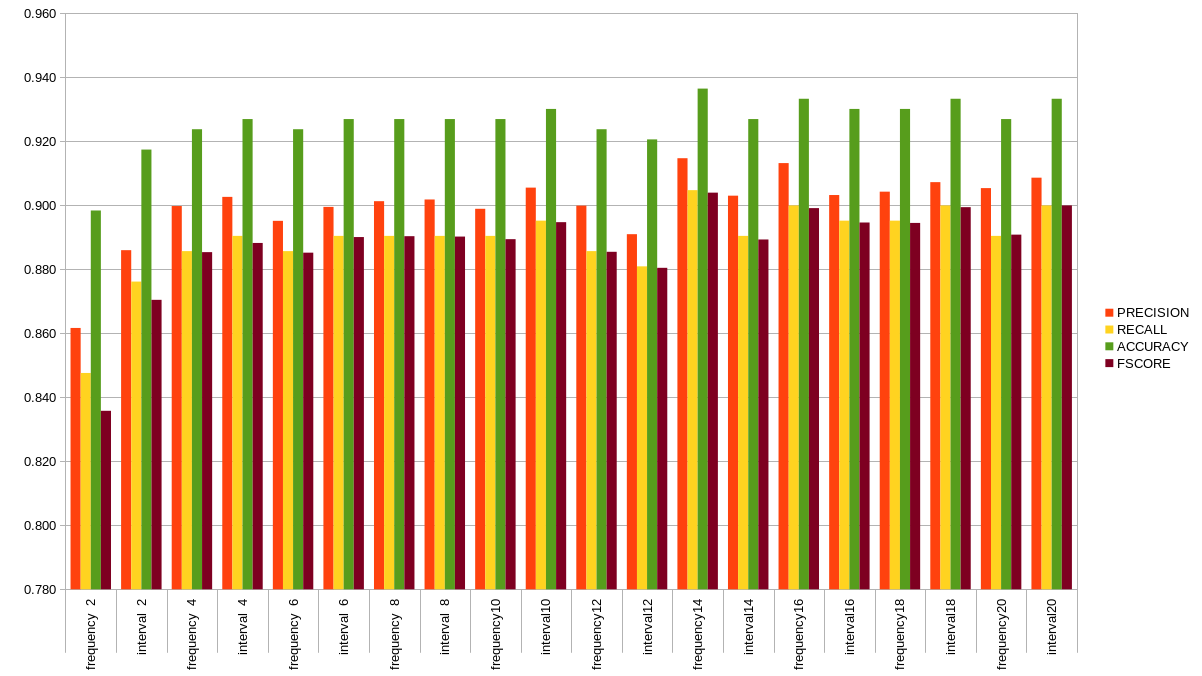
\includegraphics[width=1.0\linewidth]{disc_seeds.png}
	\caption[Wyniki klasyfikatora dla różnych metod dyskretyzacji. Zbiór seeds.]{Wyniki klasyfikatora dla różnych metod dyskretyzacji. Zbiór seeds.}
	\label{fig:disc_seeds}
\end{figure}

\subsection{Zbiór ecoli}
\begin{table}[H]
\centering
\caption{Tabela zbiór ecoli.}
\label{table-ecoli}
\begin{tabular}{llllrrrr}
METHOD    & CROSS      & AVG & SIZE & PREC & RECALL & ACCURACY & FSCORE \\
frequency & stratified & w   & 2    & nan  & 0.721  & 0.913    & nan    \\
interval  & stratified & w   & 2    & nan  & 0.712  & 0.911    & nan    \\
frequency & stratified & w   & 4    & nan  & 0.768  & 0.927    & nan    \\
interval  & stratified & w   & 4    & nan  & 0.803  & 0.941    & nan    \\
frequency & stratified & w   & 6    & nan  & 0.809  & 0.945    & nan    \\
interval  & stratified & w   & 6    & nan  & 0.815  & 0.945    & nan    \\
frequency & stratified & w   & 8    & nan  & 0.794  & 0.942    & nan    \\
interval  & stratified & w   & 8    & nan  & 0.782  & 0.940    & nan    \\
frequency & stratified & w   & 10   & nan  & 0.774  & 0.934    & nan    \\
interval  & stratified & w   & 10   & nan  & 0.765  & 0.934    & nan    \\
frequency & stratified & w   & 12   & nan  & 0.771  & 0.935    & nan    \\
interval  & stratified & w   & 12   & nan  & 0.779  & 0.938    & nan    \\
frequency & stratified & w   & 14   & nan  & 0.762  & 0.933    & nan    \\
interval  & stratified & w   & 14   & nan  & 0.756  & 0.932    & nan    \\
frequency & stratified & w   & 16   & nan  & 0.744  & 0.926    & nan    \\
interval  & stratified & w   & 16   & nan  & 0.756  & 0.931    & nan    \\
frequency & stratified & w   & 18   & nan  & 0.753  & 0.926    & nan    \\
interval  & stratified & w   & 18   & nan  & 0.744  & 0.924    & nan    \\
frequency & stratified & w   & 20   & nan  & 0.732  & 0.919    & nan    \\
interval  & stratified & w   & 20   & nan  & 0.756  & 0.926    & nan   
\end{tabular}
\end{table}

\begin{figure}[H]
	\centering
		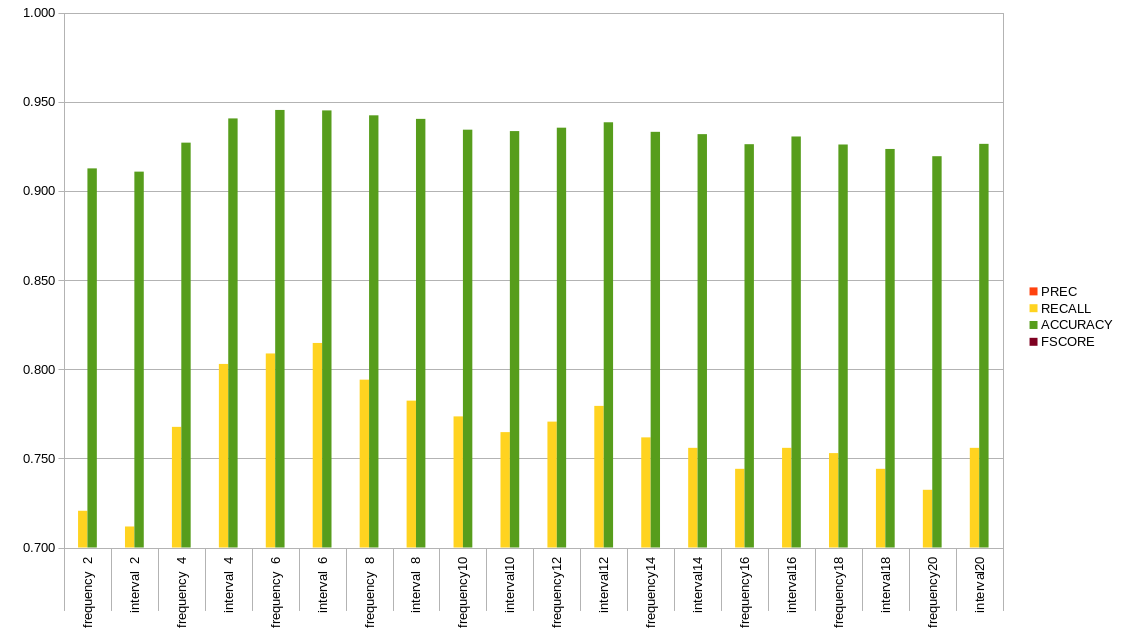
\includegraphics[width=1.0\linewidth]{disc_ecoli.png}
	\caption[Wyniki klasyfikatora dla różnych metod dyskretyzacji. Zbiór ecoli.]{Wyniki klasyfikatora dla różnych metod dyskretyzacji. Zbiór ecoli.}
	\label{fig:disc_ecoli}
\end{figure}

\subsection{Zbiór ukm}
\begin{table}[H]
\centering
\caption{Tabela zbiór ukm.}
\label{table-ukm}
\begin{tabular}{llllrrrr}
METHOD    & CROSS      & AVG & SIZE & PREC  & RECALL & ACCURACY & FSCORE \\
frequency & stratified & w   & 2    & nan   & 0.574  & 0.773    & nan    \\
interval  & stratified & w   & 2    & nan   & 0.623  & 0.800    & nan    \\
frequency & stratified & w   & 4    & 0.788 & 0.746  & 0.857    & 0.744  \\
interval  & stratified & w   & 4    & 0.845 & 0.826  & 0.905    & 0.824  \\
frequency & stratified & w   & 6    & 0.823 & 0.803  & 0.891    & 0.801  \\
interval  & stratified & w   & 6    & 0.864 & 0.851  & 0.917    & 0.851  \\
frequency & stratified & w   & 8    & 0.866 & 0.851  & 0.917    & 0.852  \\
interval  & stratified & w   & 8    & 0.867 & 0.849  & 0.917    & 0.847  \\
frequency & stratified & w   & 10   & 0.855 & 0.846  & 0.914    & 0.845  \\
interval  & stratified & w   & 10   & 0.862 & 0.841  & 0.915    & 0.839  \\
frequency & stratified & w   & 12   & 0.863 & 0.841  & 0.911    & 0.840  \\
interval  & stratified & w   & 12   & 0.861 & 0.844  & 0.913    & 0.842  \\
frequency & stratified & w   & 14   & 0.870 & 0.849  & 0.917    & 0.849  \\
interval  & stratified & w   & 14   & nan   & 0.849  & 0.918    & nan    \\
frequency & stratified & w   & 16   & 0.842 & 0.828  & 0.905    & 0.827  \\
interval  & stratified & w   & 16   & 0.841 & 0.823  & 0.902    & 0.823  \\
frequency & stratified & w   & 18   & 0.835 & 0.821  & 0.901    & 0.820  \\
interval  & stratified & w   & 18   & 0.839 & 0.815  & 0.900    & 0.814  \\
frequency & stratified & w   & 20   & 0.831 & 0.810  & 0.897    & 0.811  \\
interval  & stratified & w   & 20   & 0.843 & 0.823  & 0.902    & 0.821 
\end{tabular}
\end{table}

\begin{figure}[H]
	\centering
		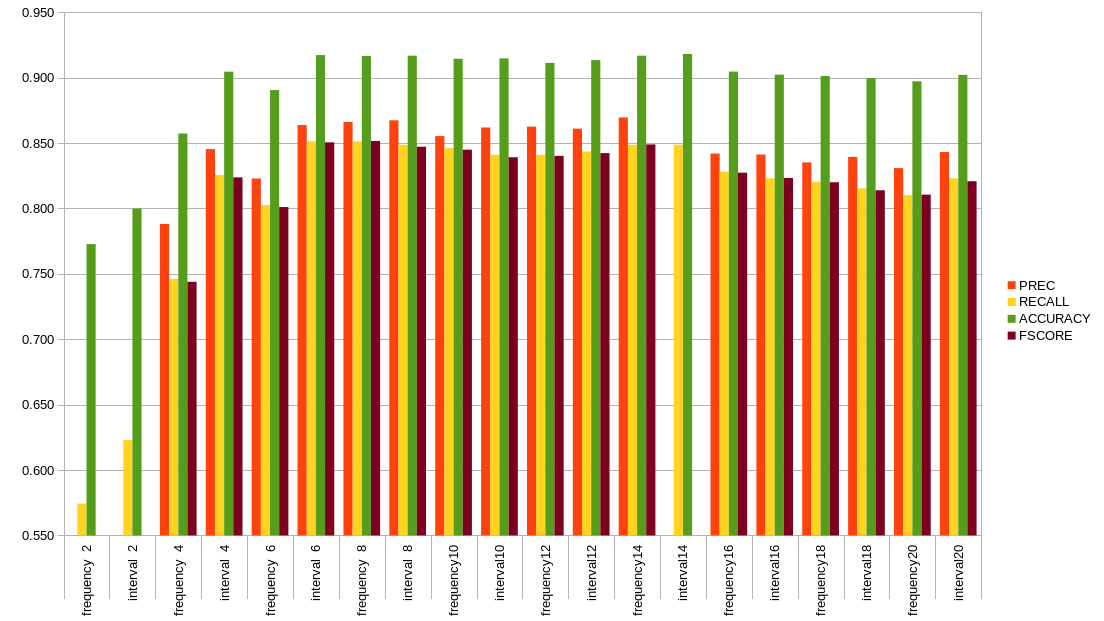
\includegraphics[width=1.0\linewidth]{disc_ukm.png}
	\caption[Wyniki klasyfikatora dla różnych metod dyskretyzacji. Zbiór ukm.]{Wyniki klasyfikatora dla różnych metod dyskretyzacji. Zbiór ukm.}
	\label{fig:disc_ukm}
\end{figure}

\section{Porównanie metod kroswalidacji}

\begin{table}[H]
\centering
\caption{Tabela kroswalidacja.}
\label{table-cross}
\begin{tabular}{lllllrrrr}
NAME  & DATASET   & CROSS      & AVG & SIZE & PREC  & RECALL & ACCURACY & FSCORE \\
ukm   & frequency & stratified & w   & 8    & 0.866 & 0.851  & 0.917    & 0.852  \\
ukm   & frequency & cross      & w   & 8    & 0.865 & 0.850  & 0.914    & 0.850  \\
ecoli & frequency & stratified & w   & 6    & nan   & 0.809  & 0.945    & nan    \\
ecoli & frequency & cross      & w   & 6    & nan   & 0.852  & 0.945    & nan    \\
seeds & frequency & stratified & w   & 14   & 0.915 & 0.905  & 0.937    & 0.904  \\
seeds & frequency & cross      & w   & 14   & 0.900 & 0.890  & 0.925    & 0.890 
\end{tabular}
\end{table}

\begin{figure}[H]
	\centering
		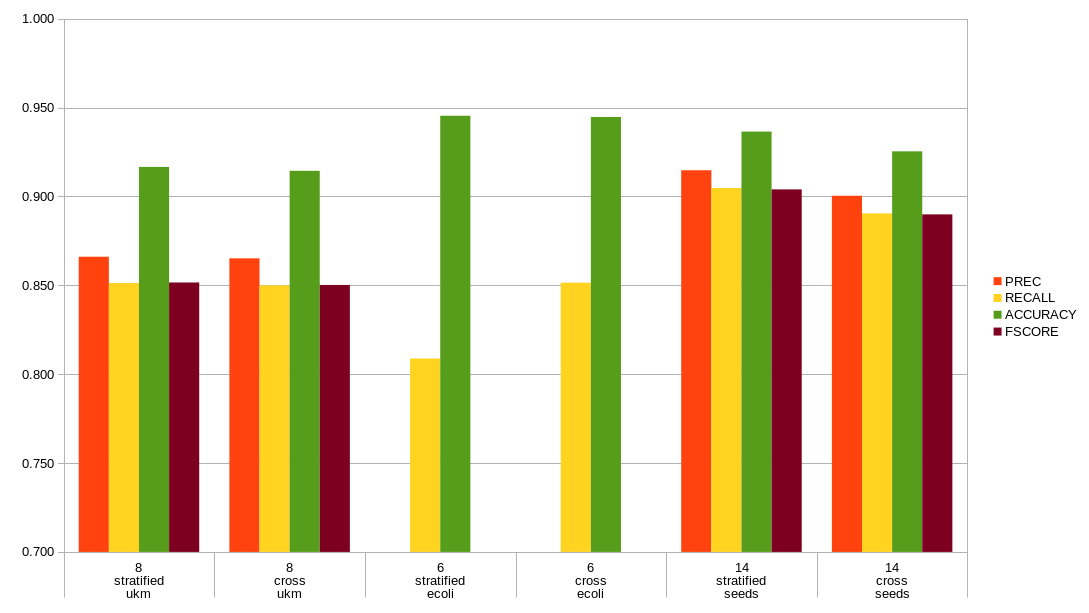
\includegraphics[width=1.0\linewidth]{cross.png}
	\caption[Wyniki klasyfikatora dla różnych metod kroswalidacji.]{Wyniki klasyfikatora dla różnych metod kroswalidacji.}
	\label{fig:cross}
\end{figure}



\section{Porównanie metod obliczenia statystyk}

\begin{table}[H]
\centering
\caption{Tabela statystyki.}
\label{table-stats}
\begin{tabular}{lllllrrrr}
NAME  & DATASET   & CROSS      & AVG & SIZE & PREC  & RECALL & ACCURACY & FSCORE \\
seeds & frequency & stratified & w   & 14   & 0.915 & 0.905  & 0.937    & 0.904  \\
seeds & frequency & stratified & u   & 14   & 0.915 & 0.905  & 0.937    & 0.904  \\
seeds & frequency & stratified & g   & 14   & 0.936 & 0.965  & 0.905    & 0.950  \\
ecoli & frequency & stratified & u   & 6    & nan   & 0.524  & 0.952    & nan    \\
ecoli & frequency & stratified & w   & 6    & nan   & 0.809  & 0.945    & nan    \\
ecoli & frequency & stratified & g   & 6    & 0.848 & 0.944  & 0.809    & 0.893  \\
ukm   & frequency & stratified & u   & 8    & 0.878 & 0.846  & 0.926    & 0.855  \\
ukm   & frequency & stratified & w   & 8    & 0.866 & 0.851  & 0.917    & 0.852  \\
ukm   & frequency & stratified & g   & 8    & 0.920 & 0.920  & 0.851    & 0.919 
\end{tabular}
\end{table}

\begin{figure}[H]
	\centering
		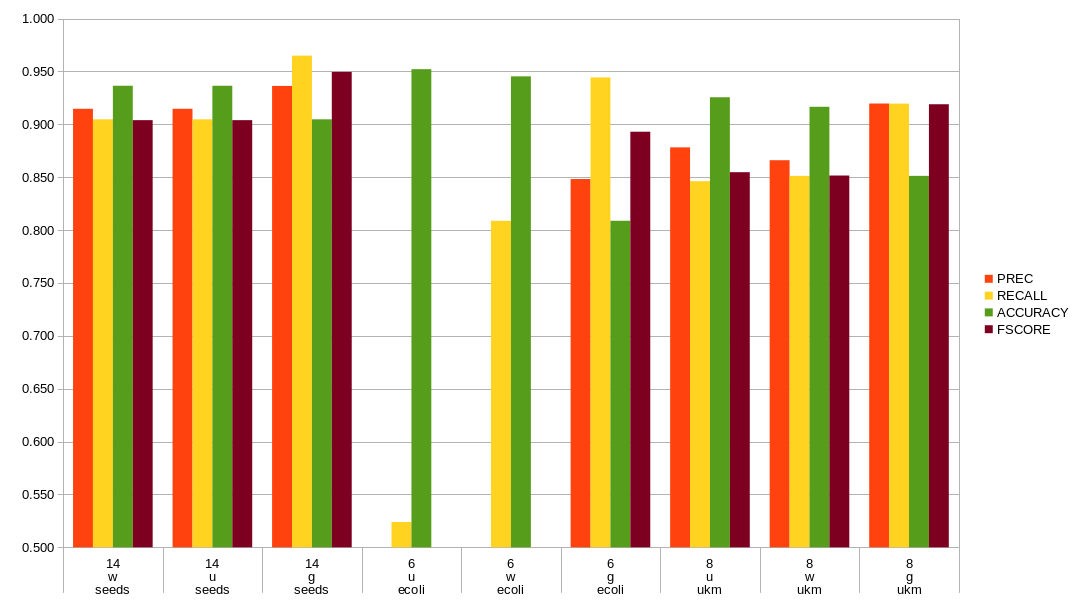
\includegraphics[width=1.0\linewidth]{stats.png}
	\caption[Wyniki klasyfikatora dla różnych metod obliczania statystyki.]{Wyniki klasyfikatora dla różnych metod obliczania statystyki.}
	\label{fig:stats}
\end{figure}

\section{Dane ciągłe}

\begin{table}[H]
\centering
\caption{Tabela dane ciągłe.}
\label{table-norm}
\begin{tabular}{lllllrrrr}
NAME  & DATASET   & CROSS      & AVG & SIZE & PREC  & RECALL & ACCURACY & FSCORE \\
seeds & frequency & stratified & w   & 14   & 0.915 & 0.905  & 0.937    & 0.904  \\
seeds & norm      & stratified & w   & -    & 0.902 & 0.876  & 0.917    & 0.877  \\
ecoli & frequency & stratified & w   & 6    & nan   & 0.809  & 0.945    & nan    \\
ecoli & norm      & stratified & w   & -    & nan   & 0.412  & 0.680    & nan    \\
ukm   & frequency & stratified & w   & 8    & 0.866 & 0.851  & 0.917    & 0.852  \\
ukm   & norm      & stratified & w   & -    & 0.880 & 0.864  & 0.924    & 0.864 
\end{tabular}
\end{table}

\begin{figure}[H]
	\centering
		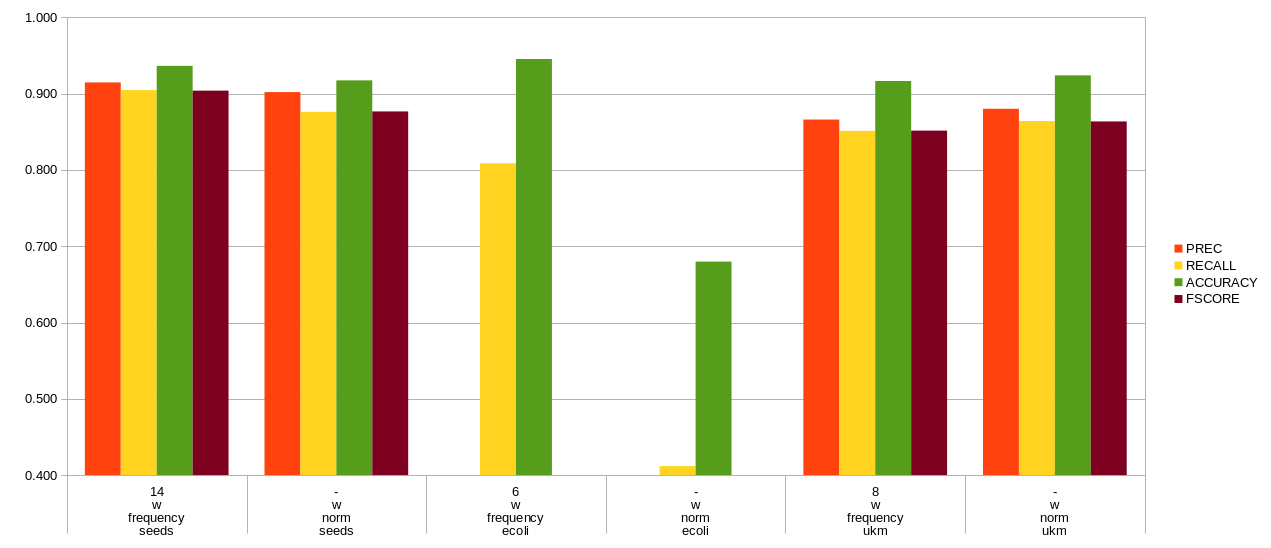
\includegraphics[width=1.0\linewidth]{norm.png}
	\caption[Porównanie wyników dyskretnych z wartościami ciągłymi.]{Porównanie wyników dyskretnych z wartościami ciągłymi.}
	\label{fig:norm}
\end{figure}
%\chapter{Prezentacja}
\section{Działanie}
Po uruchomieniu programu ukazuje się menu główne z trzema zakładkami: Home, Calibration oraz Machine learning. W zakładce Home użytkownik wybrać może wejście, które będzie przetwarzane(rys. \ref{fig:home}a). W tej zakładce można również uruchomić główną funkcjonalność programu, czyli rozpoznawanie gestów, dostępne pod przyciskiem Start recognition. Po wybraniu wejścia jako filmu wideo (rys. \ref{fig:home}b) ukazuje się menu wyboru pliku, a po uruchomieniu programu suwak regulujący prędkość przetwarzania w klatkach na sekundę. Jeśli zaznaczona zostanie opcja Max FPS, przetwarzanie obrazu będzie działać z maksymalną wydajnością.

\begin{figure}[!htpb]
	\centering

	\begin{tabular}{l l}
		a) & b) \\
		\fbox{\includegraphics[width=0.45\textwidth]{rys05/home}} &
		\fbox{\includegraphics[width=0.45\textwidth]{rys05/video}}	
	\end{tabular}
	\caption{Główne okno aplikacji.}
	\label{fig:home}
\end{figure}
\newpage
Drugą zakładką jest kalibracja (rys. \ref{fig:calib}a). W niej można dokonać zmiany opcji segmentacji obrazu. Użytkownik może wybrać pomiędzy metodami wycianania tła i progowania koloru dłoni. Dodatkowo może zapisać i załadować ustawienia. Po uruchomieniu opcji kalibracji koloru, pokazywane są trzy suwaki (rys. \ref{fig:calib}b) odpowiadające kolejnym wartością w przestrzeni HSL.

\begin{figure}[!htpb]
	\centering
	\begin{tabular}{l l}
			a) & b) \\
			\fbox{\includegraphics[width=0.45\textwidth]{rys05/calib}} &
			\fbox{\includegraphics[width=0.45\textwidth]{rys05/calib_color}}	
	\end{tabular}
	\caption[Okno kalibracji]{Okno kalibracji (po lewej) oraz kalibracja koloru (po prawej).}
	\label{fig:calib}
\end{figure}

Zakaładka Machine learning zawiera dwa przyciski (rys. \ref{fig:ml_inside}a): Start data acquisition oraz Vision. Pierwsza opcja odpowiedzialna jest za tworzenie zbioru uczącego (rys. \ref{fig:ml_inside}b), a druga do graficznej prezentacji segmentacji obrazu i tworzenia wektora cech.

\begin{figure}[!htpb]
	\centering
	\begin{tabular}{l l}
			a) & b) \\
			\fbox{\includegraphics[width=0.45\textwidth]{rys05/ml}} &
			\fbox{\includegraphics[width=0.45\textwidth]{rys05/ml_data}}	
	\end{tabular}
	\caption[Okno uczenia maszynwego i akwizycji danych] {Okno uczenia maszynwegoh (po lewej) oraz akwizycji danych (po prawej).}
	\label{fig:ml_inside}
\end{figure}
\newpage
\section{Skuteczność} \label{section:experiments}
Do eksperymentu wyróżniono zestaw 25 gestów dłoni. W tabeli \ref{table:gestures} przedstawiono ich nazwy oraz wygląd.

\newcommand{\gesture}[2]
{
#1  &  \raisebox{-0.5\totalheight}[30pt]{\includegraphics[height=30pt]{rys05/#2}}
}

\begin{table}[!htb]
\centering
\caption{Zestawienie gestów dłoni.}
\begin{tabular}{|c|c|c|c|}
\hline
\gesture{CLOSED}{closed} &
\gesture{POINTING}{pointing} \\ \hline
\gesture{MIDDLE}{middle}&
\gesture{LITTLE}{little} \\ \hline
\gesture{VICTORIA}{victoria}&
\gesture{GUN}{gun} \\ \hline
\gesture{MIDDLE GUN}{middle_gun}&
\gesture{PHONE}{phone} \\ \hline
\gesture{SNAIL}{snail}&
\gesture{THREE}{three} \\ \hline
\gesture{SATAN}{satan}&
\gesture{OKEY}{okey} \\ \hline
\gesture{MIDDLE THREE}{middle_three}&
\gesture{LITTLE VICTORIA}{little_victoria} \\ \hline
\gesture{FOUR}{four}&
\gesture{FIVE}{five} \\ \hline
\gesture{GLOVE}{glove}& 
\gesture{TWO TWO}{two_two} \\  \hline
\gesture{THREE ONE}{three_one}&
\gesture{ONE THREE}{one_three} \\ \hline
\gesture{ONE TWO ONE}{one_two_one}&
\gesture{THUMB TWO TWO}{thumb_two_two} \\ \hline
\gesture{THUMB THREE ONE}{thumb_three_one} &
\gesture{THUMB ONE THREE}{thumb_one_three} \\ \hline
\gesture{THUMB ONE TWO ONE}{thumb_one_two_one} &  &\\ \hline 
\end{tabular}
\label{table:gestures}
\end{table}
\newpage
W badaniu przetestowano 5 różnych klasyfikatorów, opisanych w rozdziale \ref{section:machine_learning}:
\begin{itemize}
	\item SVM - maszyna wektorów nośnych
	\item RFC - klasyfikator lasu drzew decyzyjnych
	\item KNN - k - najbliższych sąsiadów
	\item GNB - naiwny klasyfikator bayesowski
	\item MLP - wielowarstwowa sieć neuronowa.
\end{itemize}
Przeprowadzono przy tym dwa eksperymenty na różnej wielkości bazach. Baza postawowa składała się z 3\,482 rekordów i 7 gestów. Baza rozszerzona natomiast zawierała 37\,872 rekordów podzielonych na 25 klas przedstawionych w tabeli \ref{table:gestures}. Wyniki eksperymentu dla uproszczonego zestawu przedstawiono w tabeli \ref{table:simple_results}, a dla rozszerzonego w \ref{table:results}. Oznaczają one procentową skuteczność rozpoznania danego gestu. 

\begin{table}[!htbp]
\centering
\caption{Skuteczność klasyfikatorów - baza podstawowa.}
\label{table:simple_results}
\begin{tabular}{l|rrrrrr}
 & GNB [\%] & KNN [\%] & MLP [\%] & RFC [\%] & SVM [\%] \\ \hline
CLOSED & 95.2900 & 55.2900 & 89.4100 & 100.0000 & 60.0000 \\
POINTING & 93.2000 & 84.4700 & 89.3200 & 97.0900 & 83.5000 \\
FOUR & 90.4800 & 94.0500 & 97.0200 & 98.2100 & 90.4800 \\
FIVE & 99.4400 & 92.1300 & 94.9400 & 100.0000 & 90.4500 \\
VICTORIA & 94.9200 & 98.3100 & 98.3100 & 99.1500 & 97.0300 \\
PHONE & 90.0000 & 98.0000 & 100.0000 & 100.0000 & 98.0000 \\
THREE & 98.0400 & 94.1200 & 98.0400 & 100.0000 & 94.1200 \\
\end{tabular}
\end{table}

Najlepszym modelem klasyfikacji okazał się być las drzew decyzyjnych, który cechował się blisko 100\% skutecznością. Z drugiej strony, najsłabszymi klasyfikatorami w tym przypadku okazały się być MLP oraz GNB. W przypadku sieci neuronowych, słaba skuteczność mogła być wynikiem ustawienia złych parametrów (ilość neuronów, ilość warstw) oraz małego zestawu danych uczących. Jeśli chodzi o naiwny klasyfikator bayesowski, niska skuteczność była spowodowana tym, że wektor cech zawierał dane silnie ze sobą skorelowane, a jego działanie powinno opierać się na wektorach o elementach niezależnych od siebie.

Otrzymane wyniki wyraźnie pokazują, że w przypadku mniejszej bazy gestów, system cechuje się wyraźnie lepszą skutecznością. Podstawowy zbiór gestów zawierał gesty, które wyraźnie się od siebie różniły np. ilość wyprostowanych palców. W połączeniu ze strukturą wektora cech, modele klasyfikatorów mogły lepiej dostosować swoje parametry.

O ile dla danych testowych klasyfikatory wykazały się relatywnie wysoką skutecznością(około 95\% w przypadku bazy podstawowej i 80\% dla bazy rozszerzonej), w praktyce skuteczność ta nie jest tak wysoka. Powodem niższej skuteczności jest najprawdopodobniej zjawisko nadmiernego dopasowania (ang. overfitting), w którym model zbyt dobrze dostosował się do danych uczących. Konfiguracja, specyfika dłoni i inne cechy danych uczących znalazły się w modelu, przez co najmniejsza ich zmiana powoduje obniżenie skuteczności.

\newpage
\begin{landscape}

\begin{table}[]
\centering
\caption{Skuteczność klasyfikatorów - baza rozszerzona.}
\label{table:results}
\begin{tabular}{l|rrrrrr}
& GNB [\%] & KNN [\%] & MLP [\%] & RFC [\%] & SVM [\%] &  \\ \hline
CLOSED            & 86.6700           & 81.7500           & 64.2100           & 100.0000          & 84.5600           &  \\
POINTING          & 73.8000           & 83.0700           & 70.6100           & 100.0000          & 86.5800           &  \\
MIDDLE            & 90.0000           & 77.9300           & 30.6900           & 100.0000          & 43.7900           &  \\
LITTLE            & 80.5900           & 84.3700           & 76.8200           & 100.0000          & 84.3700           &  \\
VICTORIA          & 16.8000           & 81.0800           & 71.2400           & 99.4200           & 74.1300           &  \\
GUN               & 55.3000           & 85.2700           & 53.7500           & 100.0000          & 79.8400           &  \\
MIDDLE GUN        & 79.4200           & 87.7700           & 66.0200           & 100.0000          & 84.2700           &  \\
PHONE             & 78.3500           & 76.3800           & 64.7600           & 100.0000          & 75.5900           &  \\
SNAIL             & 97.2700           & 80.4700           & 74.0200           & 99.4100           & 79.1000           &  \\
THREE             & 45.5600           & 88.5700           & 78.9500           & 100.0000          & 86.4700           &  \\
SATAN             & 61.6000           & 82.7300           & 72.1600           & 100.0000          & 82.2200           &  \\
OKEY              & 93.2000           & 92.2800           & 83.8200           & 100.0000          & 93.7500           &  \\
MIDDLE THRE       & 76.8400           & 84.4700           & 67.3000           & 100.0000          & 78.7500           &  \\
LITLLE VICTORIA   & 90.5000           & 88.8300           & 76.9100           & 100.0000          & 81.0100           &  \\
FOUR              & 88.3000           & 94.1500           & 80.7000           & 100.0000          & 96.4900           &  \\
FIVE              & 99.4000           & 97.6200           & 93.4500           & 100.0000          & 97.6200           &  \\
GLOVE             & 98.9200           & 92.8100           & 86.3300           & 100.0000          & 91.0100           &  \\
TWO TWO           & 93.6900           & 74.7600           & 61.6500           & 100.0000          & 79.1300           &  \\
THREE ONE         & 93.1000           & 82.4100           & 72.4100           & 100.0000          & 79.3100           &  \\
ONE THREE         & 33.8500           & 88.8200           & 77.3300           & 100.0000          & 86.0200           &  \\
ONE TWO ONE       & 70.9600           & 81.7400           & 61.0800           & 100.0000          & 56.2900           &  \\
THUMB TWO TWO     & 88.8900           & 85.8600           & 75.0800           & 100.0000          & 80.4700           &  \\
THUMB THREE ONE   & 92.7200           & 87.8700           & 80.0500           & 100.0000          & 90.3000           &  \\
THUMB ONE THREE   & 75.2300           & 77.5700           & 73.8300           & 100.0000          & 71.5000           &  \\
THUMB ONE TWO ONE & 99.7500           & 98.2600           & 95.7800           & 100.0000          & 98.7600           & 
\end{tabular}
\end{table}
\end{landscape}

%\section{Wydajność}
\chapter{Podsumowanie}
\section{Wyniki}
\section{Dalszy rozwój}

%\bibliographystyle{plalpha}
\bibliographystyle{plabbrv}

%UWAGA: bibliotekę referencji należy przygotować samemu. Dobrym do tego narzędziem jest JabRef.
%       Nazwę przygotowanej biblioteki wpisuje się poniżej bez rozszerzenia 
%       (w tym przypadku jest to "dokumentacja.bib")
\bibliography{dokumentacja}
%\appendix
%\chapter{Opis załączonej płyty CD/DVD}
Tutaj jest miejsce na zamieszczenie opisu zawartości załączonej płyty.
Należy wymienić, co zawiera.
%%\include{dodatekB}
%
%\chapterstyle{noNumbered}
%\phantomsection % sets an anchor
%\addcontentsline{toc}{chapter}{Indeks rzeczowy}
%\printindex

\end{document}
